\documentclass[11pt,a4paper]{article}

\usepackage[utf8]{inputenc}
\usepackage[T1]{fontenc}
\usepackage[catalan]{babel}
\usepackage[margin=2.5cm]{geometry}
\usepackage{graphicx}
\usepackage{float}
\usepackage{xcolor}
\usepackage{hyperref}
\usepackage{titlesec}
\usepackage{fancyhdr}
\usepackage{tabularx}
\usepackage{booktabs}
\usepackage{ragged2e}
\usepackage{setspace}
\usepackage{enumitem}
\usepackage{caption}

\setstretch{1.3}
\setlength{\parindent}{0pt}
\setlength{\parskip}{6pt}
\justifying

\hypersetup{
    colorlinks=true,
    linkcolor=black,
    urlcolor=blue!50!black,
    pdftitle={Looty Dungeon 3D - Memoria},
    pdfauthor={Carolina Rodriguez Ujano i Mateus Grandolfi Albuquerque}
}

\titleformat{\section}{\Large\bfseries}{\thesection}{0.8em}{}
\titleformat{\subsection}{\large\bfseries}{\thesubsection}{0.6em}{}

\pagestyle{fancy}
\fancyhf{}
\fancyhead[L]{\small Looty Dungeon 3D}
\fancyhead[R]{\small VJ -- FIB UPC}
\fancyfoot[C]{\thepage}
\renewcommand{\headrulewidth}{0.4pt}

\begin{document}

% ----- Pagina de titulo -----
\begin{titlepage}
\centering
\vspace*{0.6cm}

% --- Logos FIB i UPC ---
% TODO: afegir els fitxers logo_fib.png i logo_upc.png dins de Memoria/captures/
% i descomentar la linia seguent (l'enunciat demana explicitament els dos logos).
% \includegraphics[height=2.2cm]{captures/logo_fib.png}\hspace{1.5cm}\includegraphics[height=2.2cm]{captures/logo_upc.png}\par
% \vspace{0.8cm}

{\Huge\bfseries Looty Dungeon 3D\par}
\vspace{0.4cm}
{\Large Exercici 3D -- VJ (Videojocs)\par}

\vspace{1.6cm}
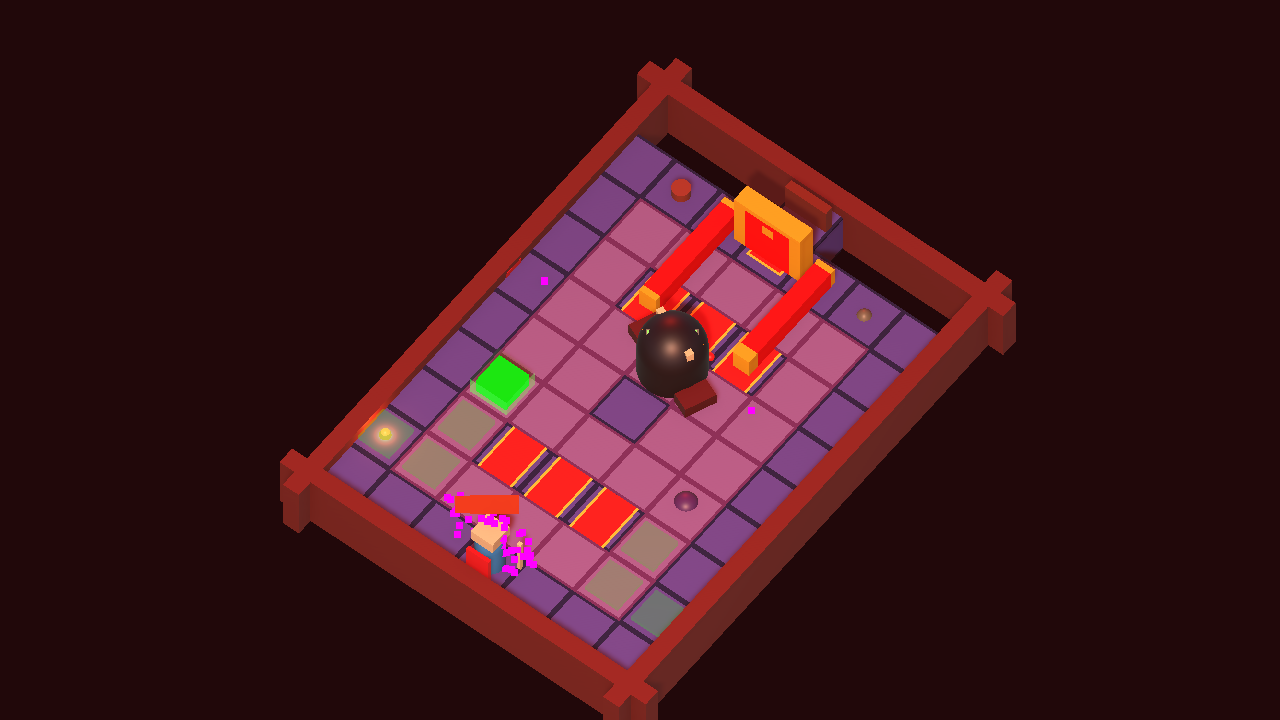
\includegraphics[width=0.55\linewidth]{captures/04_boss_room.png}\par

\vspace{1.6cm}

{\large\textbf{Autors:}\par}
{\large Carolina Rodriguez Ujano\par}
{\large Mateus Grandolfi Albuquerque\par}

\vspace{0.8cm}
{\large\textbf{Professor tutor:} Oscar Argudo Medrano\par}

\vspace{0.8cm}
{\large\textbf{Assignatura:} VJ -- Videojocs\par}
{\large\textbf{Curs:} 2025/26 (Q2)\par}
{\large\textbf{Facultat d'Informatica de Barcelona (FIB)}\par}
{\large\textbf{Universitat Politecnica de Catalunya (UPC)}\par}

\vfill
{\large \today\par}
\end{titlepage}

% ----- Index -----
\tableofcontents
\newpage

% ===== 1. El Joc =====
\section{El Joc}

\subsection{Looty Dungeon com a referencia}

El nostre projecte es basa en \textit{Looty Dungeon}, un joc \textit{rogue-lite}
de mazmorres en 3D amb perspectiva isometrica desenvolupat per
\textbf{Tinytouchtales}, publicat el 2016 per a iOS i Android i posteriorment
adaptat a altres plataformes mobils. El joc va rebre una bona acollida pel
seu estil voxel-low-poly, la seva curva de dificultat creixent i les seves
trampes ambientals.

\begin{table}[H]
\centering
\caption{Fitxa tecnica del joc original \textit{Looty Dungeon}.}
\label{tab:looty}
\begin{tabularx}{\linewidth}{lX}
\toprule
\textbf{Concepte} & \textbf{Valor} \\
\midrule
Any de publicacio & 2016 \\
Estudi & Tinytouchtales (Berlin) \\
Plataformes & iOS, Android, Windows Phone, Apple TV \\
Genere & Rogue-lite, dungeon crawler, accio-aventura \\
Public objectiu & Jugadors casuals i fans del genere mazmorrer \\
Tecnologia & Unity 5.x (motor) \\
Acollida & 4,2/5 a App Store, vora 100.000 descarregues globals \\
Web oficial & \url{https://www.tinytouchtales.com/looty-dungeon/} \\
\bottomrule
\end{tabularx}
\end{table}

La Taula~\ref{tab:looty} resumeix la fitxa del joc original. El projecte de la
nostra practica esta inspirat directament en aquest joc, simplificant-ne
algunes mecaniques pel temps disponible (3 setmanes) i adaptant-ho a un
equip de dues persones treballant en Unity 6 amb scripts en C\#.

\subsection{Equip i tecnologies}

L'equip esta format per dues persones treballant a parts iguals (Carolina
i Mateus). Hem utilitzat Unity \textbf{6000.0.74f1} amb el pipeline
\textbf{URP}, control de versions amb Git/GitHub i Visual Studio Code com a
editor. Tot el codi es propi; les referencies externes (tutorials i
documentacio) es citen a la bibliografia.

% ===== 2. Descripcio del projecte =====
\section{Descripcio del projecte}

\subsection{Objectius i trets caracteristics}

L'objectiu es desenvolupar un dungeon crawler en 3D inspirat en
\textit{Looty Dungeon} amb:

\begin{itemize}[noitemsep]
    \item 10 sales jugables amb dificultat creixent (Figura~\ref{fig:level1}).
    \item Tres enemics diferents mes un boss final.
    \item Trampes ambientals, monedes recollibles i decoracions.
    \item Caiguda de blocs per files a partir de la sala 3.
    \item Interficie grafica completa, sons i musica.
    \item Tres pantalles (menu, joc, credits) i pantalla de pausa.
\end{itemize}

\begin{figure}[H]
\centering

\includegraphics[width=0.8\linewidth]{captures/01_level1_start.png}
\caption{Vista de la primera sala. La camera ortografica isometrica esta
orientada de forma similar al \textit{Looty Dungeon} original.}
\label{fig:level1}
\end{figure}

La Figura~\ref{fig:level1} mostra la sala inicial. El jugador apareix sobre
una casella de terra de la part inferior de la sala, encarat cap a la porta
de sortida del fons.

\subsection{Instruccions de joc}

\begin{itemize}[noitemsep]
    \item \textbf{WASD} o fletxes: moure el jugador per la sala.
    \item \textbf{Shift}: dash curt per esquivar.
    \item \textbf{Espai} o \textbf{clic esquerre}: atacar.
    \item \textbf{P} o \textbf{Esc}: pausar el joc; \textbf{Enter}/\textbf{P}
    reprendre, \textbf{M} tornar al menu.
    \item Despres d'una derrota o victoria, els botons \textbf{Reintentar} /
    \textbf{Jugar de nou} reinicien la partida des de la sala 1.
    \item \textbf{0}--\textbf{9}: saltar directament a la sala corresponent.
\end{itemize}

\subsection{Diagrama de finestres i flow chart}

\begin{figure}[H]
\centering
\begin{minipage}{0.9\linewidth}
\centering
\ttfamily
\begin{tabular}{c}
\hline
{[Menu]} \\
$\downarrow$ \\
{[Credits]} $\leftrightarrow$ {[Menu]} \\
$\downarrow$ Jugar / Enter \\
{[Sala N]} -- WASD, atacs, monedes, trampes \\
$\downarrow$ \\
{[Pausa]} $\leftrightarrow$ {[Sala N]} \\
$\downarrow$ Tots els enemics morts \\
{[Porta oberta]} $\rightarrow$ {[Sala N+1]} \\
$\downarrow$ Sala 10 (boss) superada \\
{[Victoria]} $\rightarrow$ {[Menu]} \\
\quad\quad o si Vida = 0 \\
{[Game Over]} $\rightarrow$ Reintentar (sala 1) / Menu \\
\hline
\end{tabular}
\end{minipage}
\caption{Flow chart de pantalles del joc.}
\label{fig:flow}
\end{figure}

El diagrama de la Figura~\ref{fig:flow} resumeix els estats: \texttt{Menu},
\texttt{Credits}, \texttt{Playing}, \texttt{Paused}, \texttt{GameOver} i
\texttt{Victory} (gestionats per l'enum \texttt{DungeonState} de la classe
\texttt{DungeonGameRuntime}).

\subsection{Arquitectura del codi}

El projecte separa el codi en dues capes complementaries, fet que ha
facilitat el treball en paral-lel de les dues persones:

\begin{itemize}[noitemsep]
    \item \textbf{Capa d'entorn} (\texttt{LevelManager}, scripts d'enemics,
    trampes i nivells JSON): construeix la geometria de cada sala (terra,
    parets, decoracions), instancia enemics i trampes, i gestiona la caiguda
    del terra per files.
    \item \textbf{Capa de joc} (\texttt{DungeonGameRuntime} i la resta de
    scripts de \texttt{Player/}, \texttt{Game/} i \texttt{Items/}): jugador,
    combat, vida, HUD, menus, audio, camera, porta, monedes i estat global.
\end{itemize}

Les dues capes encaixen pel contracte dels enemics: el combat del jugador
crida \texttt{Hurt()} sobre els scripts d'enemic, i el runtime descobreix els
enemics que instancia el \texttt{LevelManager} per enganxar-los el feedback i
la deteccio de mort.

\subsection{Funcionalitats implementades}

\subsubsection{Mecaniques basiques}

\begin{itemize}[noitemsep]
    \item \textbf{10 sales}: definides en JSON dins \texttt{Assets/Resources/Levels/}
    (\texttt{level1.json}...\texttt{level9.json} + \texttt{final\_level.json}).
    \item \textbf{Dificultat creixent}: el nombre d'enemics, trampes i la
    presencia de blocs que cauen creix de sala en sala.
    \item \textbf{Porta condicionada}: a cada sala la porta esta tancada
    fins que tots els enemics han estat eliminats.
    \item \textbf{Tres tipus d'enemic} mes \textbf{boss}: \texttt{Slime},
    \texttt{Bat}, \texttt{Gnome} (i \texttt{Wizard}) i el \texttt{Boss} final.
    \item \textbf{Rastre ralentitzant}: el \texttt{Slime} deixa un rastre
    (\texttt{RastroSlime}) que alenteix el jugador si hi passa per sobre.
    \item \textbf{Boss multi-cop}: cal colpejar-lo diverses vegades (3 cops)
    per derrotar-lo, a diferencia dels enemics normals.
    \item \textbf{Atac del jugador} amb feedback visual i sonor; els
    enemics tambe fan dany al jugador per contacte.
    \item \textbf{Tres cors}: el jugador perd un cor per cada atac rebut
    amb exit. A zero cors es perd la partida.
    \item \textbf{Terra que cau}: a partir de la sala 3 fins a la sala 9
    (incloses), els blocs cauen per files; la sala final del boss no te
    aquesta mecanica. Els enemics que es queden sense terra a sota tambe cauen.
\end{itemize}

\subsubsection{Trampes}

S'han implementat les trampes seguents, complint amb escreix les tres
requerides per l'enunciat:

\begin{itemize}[noitemsep]
    \item \textbf{Trampa de fletxes} (\texttt{ArrowTrap} + \texttt{Arrow} +
    \texttt{Diana}): dispara fletxes que fan dany al jugador.
    \item \textbf{Forquilla retractil} (\texttt{RetractileFork}): punxes que
    surten del terra i fan dany en extendre's.
    \item \textbf{Teranyines} (\texttt{SpiderWebs}): alenteixen el jugador
    quan hi passa per sobre.
    \item \textbf{Rastre de slime} (\texttt{RastroSlime}): el rastre que deixa
    el slime i que tambe alenteix.
\end{itemize}

\subsubsection{Decoracions, monedes i interficie}

\begin{itemize}[noitemsep]
    \item \textbf{Mes de 5 decoracions diferents}: torxa de terra
    (\texttt{FloorTorch}), barril (\texttt{Barrel}), prestatgeria
    (\texttt{Bookshelf}), calder (\texttt{Cauldron}), catifa
    (\texttt{Carpet}), tapis (\texttt{Tapestry}), tron (\texttt{Throne}) i
    calze (\texttt{Caliz}). No s'hi inclouen les parets que delimiten la sala.
    \item \textbf{Monedes} (\texttt{CoinPickup}), repartides sobre el terra de
    cada sala, i \textbf{cors de vida} (\texttt{HealthPickup}, 18\,\% de
    probabilitat de drop en derrotar un enemic si la vida es inferior a 3).
    \item \textbf{Interficie}: vida amb tres cors, comptador de monedes, sales
    superades, sala actual, cronometre i barra grafica de progres de les
    10 sales (Figura~\ref{fig:level9}).
    \item \textbf{Pantalles}: menu, credits, joc, pausa, derrota i victoria.
    \item \textbf{Audio}: musica procedural per al menu, joc i boss, mes
    diversos efectes de so sintetitzats en runtime.
    \item \textbf{Tecles 0--9}: salt directe a la sala corresponent per
    facilitar l'avaluacio i el debug.
\end{itemize}

\begin{figure}[H]
\centering
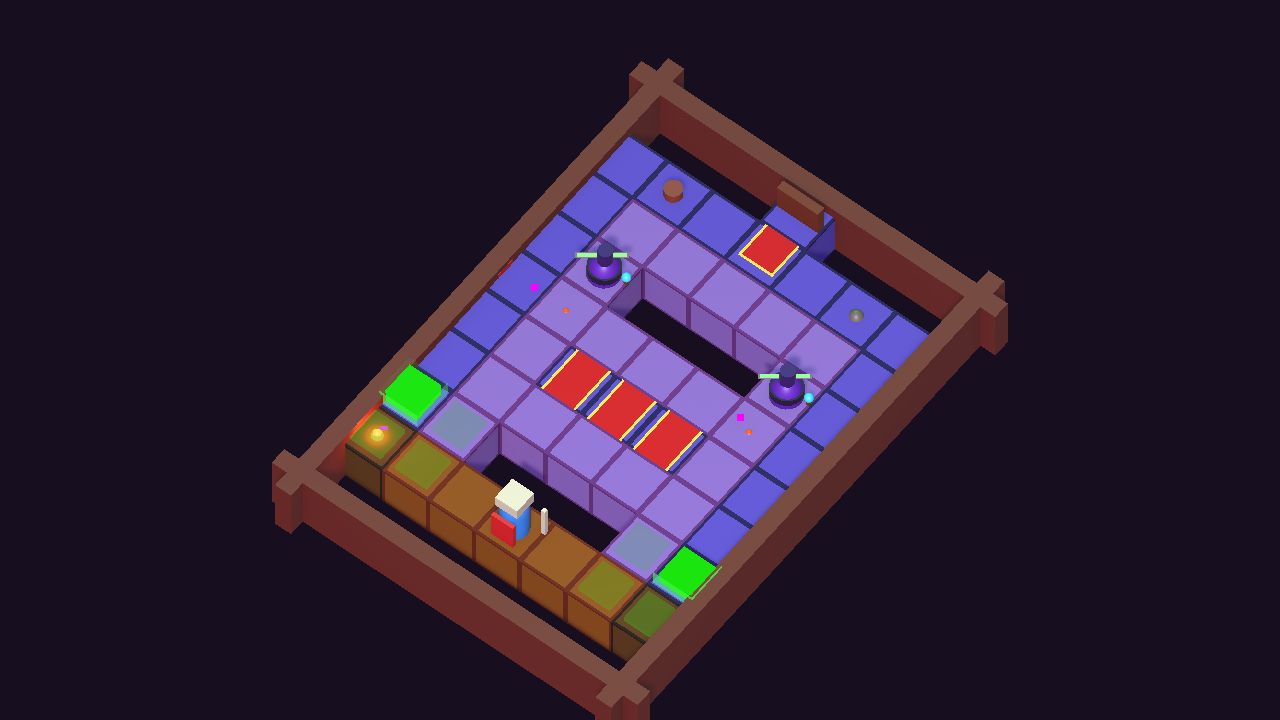
\includegraphics[width=0.8\linewidth]{captures/03_level9_falling_floor.png}
\caption{Sala amb el terra caient per files. L'indicador de progres del HUD
mostra les sales completades.}
\label{fig:level9}
\end{figure}

La Figura~\ref{fig:level9} il-lustra la mecanica de terra caient: les peces
es marquen amb un parpadeig abans de col-lapsar, avisant el jugador.

\subsubsection{Game Feeling}

S'ha posat especial cura en el feedback visual i sonor per evitar la
desaparicio instantania d'entitats:

\begin{itemize}[noitemsep]
    \item Atacs amb \textit{slash} visual, \textit{shake} de camera i sons
    diferenciats segons impactin o no.
    \item Cops a enemics amb \textit{flash}, barra de vida, text flotant de
    dany i particules.
    \item Mort d'enemics amb retard, esclat de particules i text.
    \item Dany al jugador amb parpadeig, \textit{overlay} vermell als bords i
    \textit{shake} de camera.
    \item Porta amb canvi de material, esclat de particules, text ``OPEN'' i
    so dedicat en obrir-se.
    \item Monedes i cors amb rotacio, flotacio i feedback en recollir-los.
    \item Terra caient amb avis previ, animacio de caiguda i so.
    \item Transicio amb fundit a negre entre sales.
    \item Banner de seccio en entrar a un nou bloc de la mazmorra i ambient
    (camera, llum) diferenciat per seccio (Figura~\ref{fig:traps}).
\end{itemize}

\begin{figure}[H]
\centering

\includegraphics[width=0.8\linewidth]{captures/02_level6_traps.png}
\caption{Sala intermedia amb trampes i decoracions. L'ambient es mes calid
que a les sales inicials.}
\label{fig:traps}
\end{figure}

\subsection{Decisions de disseny}

Algunes decisions concretes que hem pres o desestimat:

\begin{itemize}[noitemsep]
    \item \textbf{Pres:} usar JSON per definir les sales a
    \texttt{Assets/Resources/Levels/}, fent l'edicio rapida sense necessitat
    de recompilar.
    \item \textbf{Pres:} generar alguns visuals (jugador i enemics sense model
    propi) en runtime amb primitius (\texttt{PlayerVisualBuilder},
    \texttt{EnemyVisualBuilder} / \texttt{RuntimeEnemySetup}) i materials URP
    procedurals, evitant dependencies d'assets pesats i permetent prototipar
    el joc sencer abans de tenir tots els models finals.
    \item \textbf{Pres:} mantenir l'estil voxel/low-poly per coherencia
    estetica, tant en els assets modelats (terra, tron, torxa, calze, barril,
    prestatgeria...) com en els visuals procedurals.
    \item \textbf{Pres:} drop ocasional de cors (18\,\%) per donar marge
    d'error sense trivialitzar el joc.
    \item \textbf{Desestimat:} sistema de \textit{leaderboard} online.
    Substituit per persistencia local de la millor partida amb
    \texttt{PlayerPrefs}.
    \item \textbf{Desestimat:} sistema d'inventari/objectes consumibles, que
    hauria ampliat l'abast mes enlla del temps disponible.
\end{itemize}

% ===== 3. Metodologia =====
\section{Metodologia}

\subsection{Organitzacio del treball}

L'equip s'ha repartit la feina entre Carolina i Mateus seguint el patro del
PDF de l'enunciat (colors verd i vermell), on Carolina s'encarrega de les
sales parells i del boss, i Mateus de les sales senars. Les tasques de
Carolina han estat:

\begin{itemize}[noitemsep]
    \item Disseny de les sales parells (2, 4, 6, 8) i de la sala final del
    boss; modelat 3D dels assets (terra, parets, tron, torxa, calze, barril,
    prestatgeria, calder, catifa, tapis).
    \item Scripts d'enemics base (\texttt{Slime}, \texttt{Bat},
    \texttt{Wizard}, \texttt{Gnome}, \texttt{Boss}) i del rastre del slime.
    \item Trampes (\texttt{ArrowTrap}, \texttt{Arrow}, \texttt{Diana},
    \texttt{SpiderWebs}, \texttt{RetractileFork}) i el \texttt{LevelManager}.
    \item Logica de caiguda del terra per files al \texttt{LevelManager}.
\end{itemize}

Tasques de Mateus:

\begin{itemize}[noitemsep]
    \item Disseny de les sales senars (1, 3, 5, 7, 9).
    \item Runtime jugable (\texttt{DungeonGameRuntime}) amb estat global, HUD,
    menus, pausa, derrota, victoria i transicions.
    \item Combat del jugador (\texttt{PlayerMovement}, \texttt{PlayerCombat},
    \texttt{PlayerHealth}) i feedback (\texttt{EnemyHitFeedback}, particules,
    \textit{shake}, textos flotants).
    \item Camera ortografica isometrica i sistema de llum/ambient.
    \item Audio procedural (musica i SFX).
    \item Pickups (\texttt{CoinPickup}, \texttt{HealthPickup}) i porta.
\end{itemize}

\subsection{Planificacio i versions}

Hem dividit la feina en tres iteracions de poc mes d'una setmana cadascuna:

\begin{table}[H]
\centering
\caption{Iteracions principals del projecte.}
\label{tab:iters}
\begin{tabularx}{\linewidth}{lXl}
\toprule
\textbf{Iteracio} & \textbf{Contingut} & \textbf{Estat} \\
\midrule
1 -- Base
& Setup Unity, scripts d'enemics, slime amb rastre i disseny de les
sales basiques.
& Tancada \\
2 -- Mecaniques
& Combat, vida, HUD, porta condicionada, monedes, audio, trampes i
terra caient.
& Tancada \\
3 -- Integracio i polish
& Integracio de les dues capes a \texttt{develop}, prefabs d'enemics,
ambient per seccio, musica de boss, pickup de cor i memoria.
& En curs \\
\bottomrule
\end{tabularx}
\end{table}

La Taula~\ref{tab:iters} resumeix les iteracions.

% TODO (metodologia): l'enunciat demana captures reals de la planificacio.
% Afegir aqui imatges del diagrama de Gantt, dels sprints amb backlog
% (forecast / to-do / in-progress / done) i del seguiment de tasques
% (Trello/Slack), a mes de captures del git (historial de commits / branques).

\subsection{Repositori i seguiment}

El codi viu a \url{https://github.com/carolina-rouj/VJ-3D}. Cada membre te una
branca propia (\texttt{mateus}, \texttt{carol-...}) i fem \textit{pull request}
cap a la branca \texttt{develop} en cada fita. L'historial de commits es fa
servir com a registre temporal del treball.

% ===== 4. Conclusions =====
\section{Conclusions}

Hem desenvolupat un dungeon crawler 3D complet inspirat en \textit{Looty
Dungeon}, amb les 10 sales, els tres tipus d'enemic mes el boss, les trampes,
les monedes, el terra caient i totes les pantalles requerides. A mes dels
requisits basics, hem invertit temps en el \textit{game feel}: feedback
continu en atacs, cops i morts, transicions suaus, ambient diferenciat per
seccio i musica dedicada per al boss.

La decisio d'arquitectura que mes ens ha ajudat ha estat separar el codi en
una \textbf{capa d'entorn} (\texttt{LevelManager} i geometria) i una
\textbf{capa de joc} (\texttt{DungeonGameRuntime}, jugador, HUD i flow). Aixo
ens ha permes treballar en paral-lel i integrar les dues parts sense que una
trenques l'altra.

La principal dificultat ha estat la incompatibilitat de materials exportats
des de MagicaVoxel amb el pipeline URP de Unity 6, resolta substituint en
runtime els materials per equivalents URP-Lit. Tambe ha estat util la
generacio procedural d'entitats, que ens ha permes prototipar el joc sencer
abans de tenir tots els assets finals. Com a feina futura queden el poliment
de la IA dels enemics (persecucio i atac) i del comportament del boss.

% ===== 5. Bibliografia =====
\section{Bibliografia}

\begin{itemize}
    \item \textbf{Tinytouchtales -- Looty Dungeon}.
    \url{https://www.tinytouchtales.com/looty-dungeon/}.
    Web oficial del joc de referencia.

    \item \textbf{Unity Manual -- Universal Render Pipeline}.
    \url{https://docs.unity3d.com/Packages/com.unity.render-pipelines.universal@17.0/manual/index.html}.
    Documentacio oficial de URP per a Unity 6, utilitzada per a la
    configuracio de materials i llum.

    \item \textbf{Unity Scripting API}.
    \url{https://docs.unity3d.com/ScriptReference/}.
    Referencia oficial dels metodes del motor utilitzats al codi.

    \item \textbf{Disney -- Illusion of Life}.
    \url{https://vimeo.com/93206523}.
    Video sobre principis d'animacio que ens ha guiat la part de
    \textit{game feel}.

    \item \textbf{MagicaVoxel}.
    \url{https://ephtracy.github.io/}.
    Editor de models de voxels emprat per generar els assets 3D.
\end{itemize}

\end{document}
